
\chapter{编队网络模型和拓扑分析}
\label{chap:2}

\section{机器人编队网络模型}
在多机器人编队控制过程中,每个机器人个体都具有自主行动能力。尤其在实现分布式控制算法时,每个个体机器人需要具有独立的决策与执行能力。因此,机器人个体运动模型对编队的控制至关重要。另外在应用编队控制算法对整个编队系统进行控制从而实现特定任务时,对整体编队网络拓扑模型的掌握也是必不可少。编队网络拓扑模型是对整体编队网络拓扑分析与拓扑控制的基础\supercite{张飞2010}。

\subsection{机器人个体运动模型}
假设在$N$维空间内,机器人$R_i$的位置和速度分别表示为$p_i \in R^N$和$v_i \in R^N$。则机器人个体运动模型可以表示如下:
\begin{equation}
	\left\{
	\begin{aligned}
		\dot{p_i} & = v_i \\
		\dot{v_i} & = u_i^e + u_i^o
	\end{aligned}
	, i=1,2,\dots,n,
	\right.
\end{equation}
其中$u_i^e$表示外部对机器人的控制输入,$u_i^o$表示其他机器人对机器人$R_i$的影响。$u_i^e$可简单表示为:
\begin{equation}
	u_i^e = f(p_i,v_i), i=1,2,\dots,n
\end{equation}
若考虑障碍环境中,则$u_i^e$可表示为:
\begin{equation}
	\label{eq:outside_control}
	u_i^e = f_a(p_i,v_i) + f_r(p_i,v_i), i=1,2,\dots,n
\end{equation}
其中,$f_a(p_i,v_i)$表示来自目标的吸引力,$f_r(p_i,v_i)$表示来自障碍物的排斥力。如果已知目标点的位置$T$和机器人当前位置的期望速度$v(t)$,则$f_a(p_i,v_i)$可以表示为:
\begin{equation}
	\label{eq:object_control}
	f_a(p_i,v_i) = a_a(T-p_i) + a_m(v(t)-v_i), i=1,2,\dots,n
\end{equation}
$a_a,a_m$分别为位置和速度的增益系数,且满足$a_a,a_m > 0$。

假设环境中存在一球形障碍物,其中心点位于$O$,半径为$r_0$,则排斥力$f_r(p_i,v_i)$可表示为:
\begin{equation}
	f_r(p_i,v_i) = \begin{cases}
		\frac{a_0}{{(\lvert\lvert p_i-O \rvert\rvert -r_0)}^2} \cdot \vec{r}_t, & \lvert\lvert O-p_i \rvert\rvert \leq r_0 + R_s \\
		0, &  \lvert\lvert O-p_i \rvert\rvert > r_0 + R_s
	\end{cases}
\end{equation}
其中$a_0$为排斥系数,$R_s$为人为设置的障碍物有效作用半径。$\vec{r}_t$为排斥力的方向,即$\vec{r}_t = \vec{Op_i}/\lvert\lvert\vec{Op_i}\rvert\rvert$。
\subsection{多机器人编队网络拓扑模型}
本文的拓扑结构采用基于图论的网络拓扑。假设机器人编队中有$n$个机器人,$n$个机器人组成的编队网络用$G=(V,E)$表示,其中$V$表示图中节点的集合,$E$表示节点间边的集合。每个节点$v_i\in V, i=1,2,\dots,n$表示机器人$R_i$, $(v_i,v_j)\in E, i,j=1,2,\dots,n$表示机器人$R_i,R_j$之间的链接。利用矩阵$A=(a_{ij}),a_{ij} \in R^{n \times n}$表示网络拓扑的耦合关系,其中
\begin{equation}
	a_{ij}=a_{ji} =
	\begin{cases}
		1, & (v_i,v_j) \in E \\
		0, & (v_i,v_j) \notin E
	\end{cases}
	, i,j = 1,2,\dots\dots,n, i \neq j
\end{equation}
$a_{ij} = a){ji} = 1$ 表示机器人$i,j$之间存在有效链接,否则不存在链接。耦合矩阵对角线上的元素$a_{ij} = -\sum_{i=1,i \neq j}^n a_{ij}$。规定与机器人$R_i$存在有效连接的机器人属于机器人$R_i$的邻居。则定义机器人$R_i$的邻居集合$N_e(R_i)$为:
\begin{equation}
	N_e(R_i) = \left\{ \forall R_j, R_j \neq R_i \wedge a_{ij}=1 \right\}
\end{equation}
机器人$R_i$的度为:
\begin{equation}
	R_i.Deg = \sum_{R_j \in N_e(R_i)} a_{ij}
\end{equation}
由此可知,耦合矩阵对角线上的元素$a_{ii} = -R_i.Deg$。

多机器人编队网络拓扑多采用$K$邻居模型\supercite{xue2004number}描述。在K邻居模型中,每个机器人的度$R_i.Degree \leq K, i=1,2, \dots ,n$。图\ref{fig:K邻居网络拓扑模型}展示了几种常见的$K$邻居网络拓扑模型。
\begin{figure*}[!htbp]
	\centering
	\begin{tabular}{lr}
		\subfigure[K=3]{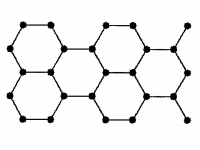
\includegraphics[width=5cm,height=4cm]{chapter2/figure2-1a.png}} &
		\subfigure[K=4]{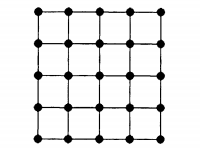
\includegraphics[width=5cm,height=4cm]{chapter2/figure2-1b.png}} \\
		\subfigure[K=6]{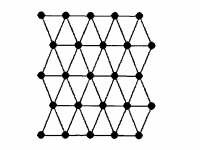
\includegraphics[width=5cm,height=4cm]{chapter2/figure2-1c.png}} &
		\subfigure[K=8]{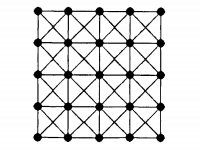
\includegraphics[width=5cm,height=4cm]{chapter2/figure2-1d.png}} \\
	\end{tabular}
	\bicaption[fig:K邻居网络拓扑模型]{几种常见的K邻居网络拓扑模型}{几种常见的K邻居网络拓扑模型}{Fig}{Several types of K-neighbor topology model.}
\end{figure*}

\section{编队网络运动同步性分析与切换控制}

\subsection{同步性理论分析}
多机器人编队网络可以看成是$N$个同样的线性耗散耦合节点的复杂动态网络,则可以用以下状态方程描述\supercite{li2003synchronization}:
\begin{equation}
	\dot{x}_i = f(x_i) + c\sum_{j=i,j \neq i}^N a_{ij}\Gamma (x_j - x_i), i=1,2,\dots,N
\end{equation}
式中$\Gamma = diag(1,\dots,1)$。当机器人$R_i$和机器人$R_j$之间存在有效链接时,$a_{ij} = a_{ji} = 1$; 否则,$a_{ij} = a_{ji} = 0$。所以有:
\[
\sum_{j=1}^N a_{ij} = \sum_{j=1}^N a{ji} = k_i
\]
另$a_{ii} = -k_i$,则上述状态方程可以简化为:
\begin{equation}
	\dot{x}_i = f(x_i) + c\sum_{j=1}^N a_{ij}x_j, i=1,2,\dots,N 
\end{equation}
当利用耦合矩阵$A = (a_{ij} \in R^{N \times N})$表征多机器人编队网络耦合关系时,由\parencite{li2003synchronization}可知,矩阵$A$的最大特征值$\lambda_1 = 0$, 其他特征值满足:
\[
	0 = \lambda_1 > \lambda_2 \geq \lambda_3 \geq \dots \geq \lambda_N
\]

当耦合网络(2-10)达到同步时,各个状态满足:
\begin{equation}
	x_1(t) = x_2(t) = \dots = x_N(t) \rightarrow s(t), t \rightarrow \infty
\end{equation}
则网络状态方程变为$\dot{S}_t = f(s(t))$。

对于动态网络$\dot{x}_i = f(x_i) + c\sum_{j=1}^N a_{ij}\Gamma (x_j-x_i), i=1,2,\dots,N$如果存在$n \times n$ 的对角阵$D>0$,以及两个常量$\bar{d}<0$和$\tau>0$,则满足:
\begin{equation}
	{\left[ Df(s(t))+dI\right]}^TD + D\left[Df(s(t)) + dI\right] \leq -\tau I
\end{equation}
$\forall d \leq \bar{d}, Df(s) \in R^{n \times n}$ 表示$f$在$s(t)$的雅克比矩阵,则如果$c\lambda_2 \leq \bar{d}$, 网络同步状态指数稳定。即
\begin{equation}
	c \geq |\frac{\bar{d}}{\lambda_2}|
\end{equation}
考虑单个机器人的动态性能,则可以另$c \geq \frac{h_{max}}{|\lambda_2|}$, $h_{max}$为网络中个体的最大李雅普诺夫指数,$h_{max}>0$。$c$代表耦合强度, $c$的取值范围越广,网络同步性的稳定性和鲁棒性越好。

由以上结论可知,
\begin{lem}
\label{lem:lambda2}
	耦合矩阵A的第二大特征值$\lambda_2$用于衡量编队网络同步的稳定性和鲁棒性。$\lambda_2$越小,编队网络同步的稳定性和鲁棒性越好,且当$\lambda_2 = 0$时,认为网络分裂成两个或多个不相连的部分\supercite{li2003synchronization}。
\end{lem}

\subsection{编队中机器人缺失对运动同步性的影响}
多机器人编队网络拓扑耦合矩阵的第二大特征值$\lambda_2$用来衡量网络的运动同步性。编队中机器人缺失会影响网络拓扑的耦合矩阵,因此会影响编队网络的与运动同步性。文献\parencite{张飞2008移动机器人覆盖问题的研究}中指出机器人缺失对编队网络同步性的影响程度大小与缺失机器人的度以及缺失机器人数量相关。图\ref{fig:sec_eigenvalue and failure ratio}显示了在丢失编队中不同度机器人的情况下,耦合矩阵第二大特征值$\lambda_2$和机器人缺失率$\Delta$的关系(缺失率:缺失机器人个数与编队总机器人个数的比值)。
\begin{figure}[!htbp]
	\centering
	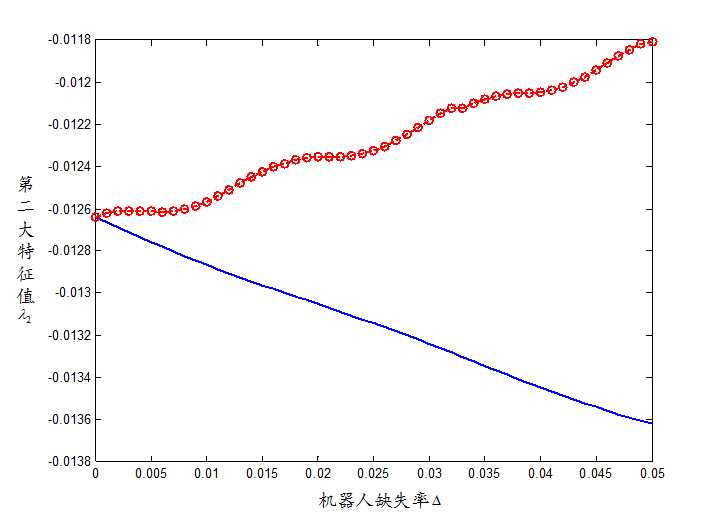
\includegraphics[width=8cm,height=6cm]{chapter2/figure2-2.png}
	\bicaption[fig:sec_eigenvalue and failure ratio]{耦合矩阵第二大特征值与缺失率变化关系}{耦合矩阵第二大特征值与缺失率变化关系。其中圆圈表示每次移除网络中度最高的机器人,实线表示每次移除网络中度最低的机器人\supercite{张飞2008移动机器人覆盖问题的研究}。}{Fig}{The relation between second-largest eigenvalue of the coupling matrix and ratio of the failed robots. The circle line means removing the highest degree robot every time, the full line means removing the lowest degree robot every time.}
\end{figure}
从图\ref{fig:sec_eigenvalue and failure ratio}可知,网络拓扑耦合矩阵的第二大特征值随网络中度最高机器人的缺失数量的增加而增大,随网络中度最低机器人的缺失数量的增加而减小。由此可知,移除编队中度最高的机器人会使编队网络运动同步性下降,移除编队中度最低的机器人会使编队网络的运动同步性提高。

从矩阵层面考虑度的大小与编队运动同步性的关系,则耦合矩阵$A$的一般形式:
\begin{equation}
	A = 
	\begin{bmatrix}
		-d_1 & 1 & 0 & \dots & 0 \\
		1 & -d_2 & 0 & \dots & 0 \\
		0 & 0 & -d_3 & \dots & 0 \\
		\vdots & \vdots & \vdots & \vdots & \vdots\\
		0 & 0 & 0 & \dots & -d_n
	\end{bmatrix}
\end{equation}
根据矩阵与图论的相关理论可知,耦合矩阵$A$的第二大特征值随着机器人的度$R_i.Deg, i=1,2,\dots,n$的增加而减小。也就是说机器人度的增加会提高编队的运动同步性\supercite{张飞2008移动机器人覆盖问题的研究}。根据以上研究可得出结论:
\begin{lem}
	\label{lem:degree_syn}
	当机器人编队网络中出现缺失机器人时,用度较低的机器人代替度较高的缺失机器人可以改善编队运动同步性,且机器人的度提升的越多,同步性改善程度越大。
\end{lem}
本文的自修复算法主要是依据引理\ref{lem:degree_syn}进行设计。为实现同步性改善的全局最优,当编队中出现机器人缺失时,利用编队中度最小的机器人去替换缺失机器人。

\subsection{编队递归拓扑切换控制}
当编队中出现机器人缺失时,最简单的方法就是指派编队中度最小的机器人去填补缺失机器人的空缺。如图\ref{fig:拓扑切换控制}(a)所示。
\begin{figure*}[!htbp]
	\centering
	\begin{tabular}{c}
		\subfigure[直接拓扑切换控制]{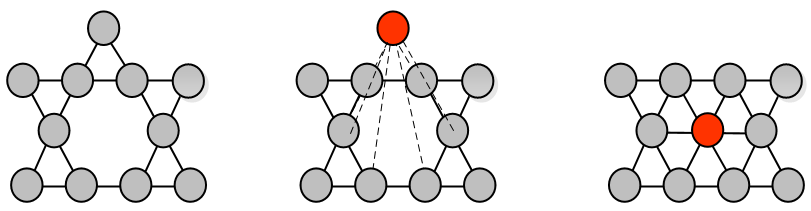
\includegraphics[width=10cm,height=3cm]{chapter2/figure2-3a.png}}\\
		\subfigure[递归拓扑切换控制]{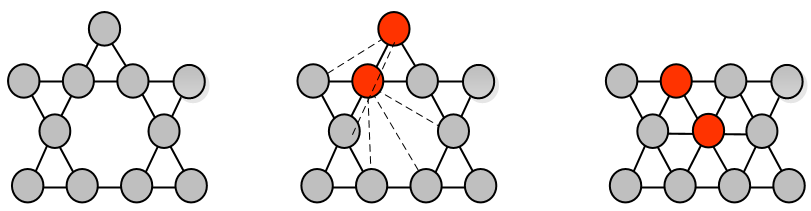
\includegraphics[width=10cm,height=3cm]{chapter2/figure2-3b.png}}
	\end{tabular}
	\bicaption[fig:拓扑切换控制]{直接拓扑切换控制与递归拓扑切换控制过程比较}{直接拓扑切换控制与递归拓扑切换控制过程比较。}{Fig}{The comparation between directly-switched topology control and recursively-switched topology control.}
\end{figure*}
然而,要想实现图中所示的直接自修复效果,需要集中式控制。但对于多机器人编队系统,集中式控制在个体机器人控制,算法实现,可扩展性等方面存在一定的局限性。并且修复机器人的运动距离过长,能量消耗过多,后期可能会由于能量不足无法与编队中其他机器人保持同步。

鉴于直接拓扑切换控制方法的各种问题,本文算法的拓扑切换方式采用递归拓扑切换控制,如图\ref{fig:拓扑切换控制}(b)所示。
编队中出现机器人缺失后,缺失机器人的空缺由其邻居中的某个机器人填补,填补空缺的机器人留下的新的空缺则再由其邻居中的机器人填补,重复执行此过程直到最后编队中度最小机器人填补了空缺。最终修复效果与直接拓扑切换控制等效,但相比于直接拓扑切换控制,递归拓扑切换控制只需要邻居间的机器人互相通信,通信距离较短,抗干扰能力更强,易于实现分布式。同时机器人的移动距离较短,功率消耗较少。因此,本文采用递归拓扑切换控制方式实现自修复过程。

\section{本章小结}
本章主要介绍了多机器人编队网络模型和拓扑结构分析。对于多机器人编队网络模型,主要从机器人个体运动模型和编队网络拓扑模型两个层面分析。在个体运动模型方面,给出机器人运动的状态描述方程。在编队网络拓扑模型方面给出了描述拓扑结构的图模型及耦合矩阵,并定义了机器人度的概念,同时介绍了几种K邻居拓扑模型。网络拓扑分析方面,主要论证了耦合矩阵的第二大特征值可以用来衡量编队的同步性。且通过分析编队中机器人缺失对网络同步性的影响,得出利用编队中度最小的机器人替换度较高的缺失的机器人可以实现同步性改善全局最优的结论。最后对比分析了直接拓扑切换与递归拓扑切换两种拓扑切换方式的优缺点,本文采用递归拓扑切换方式实现自修复过程。